\chapter{Исследовательская часть}
\section{Технические характеристики}
Тестирование выполнялось на устройстве со следующими техническими характеристиками:
\begin{itemize}
	\item Операционная система Pop!\_OS 22.04 LTS \cite{ubuntu} Linux \cite{linux};
	\item Оперативная память 16 Гб;
	\item Процессор AMD® Ryzen 7 2700 eight-core processor × 16 \cite{amd}.
\end{itemize}

Во время тестирования устройство было подключено к блоку питания и не нагружено никакими приложениями, кроме встроенных приложений окружения, окружением и системой тестирования.

\section{Демонстрация работы программы}



На рисунке \ref{demonstration} представлен результат работы программы, в которой выводится время работа алгоритма и количество найденных кластеров.

\begin{figure}[ht!]
	\begin{center}
		\captionsetup{singlelinecheck = false, justification=centerfirst}
		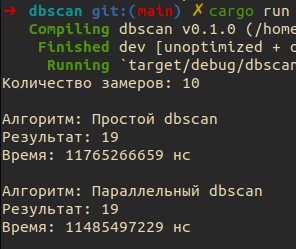
\includegraphics[scale=0.8]{assets/demonstration.png}
		\caption{Пример работы программы}
		\label{demonstration}
	\end{center}
	
	
\end{figure}

\newpage

\section{Время выполнения реализации алгоритмов}

Результаты замеров времени работы реализаций алгоритмов DBSCAN (в с) приведены в таблице \ref{tbl:best}. Сравнение проводилось между простым алгоритмом и параллельного алгоритма при исполнении на 8 потоках.
\newcolumntype{d}[1]{D{.}{.}{-1}}
\begin{table}[ht!]
	\begin{center}
			\captionsetup{justification=raggedright,singlelinecheck=off}
			\caption{Результаты замеров реализаций алгоритмов DBSCAN}
			\label{tbl:best}
			\begin{tabular}{|c|d{6.3}|d{6.3}|}
				\hline
				Размер & \multicolumn{1}{c|}{\text{Простой DBSCAN}} &  \multicolumn{1}{c|}{\text{Параллельный DBSCAN}}  \\
				\hline
				100 & 11.765266659 & 11.485497229 \\ 
				\hline
				200 & 25.211357678 & 21.986658269 \\ 
				\hline
				300 & 43.935717611 & 40.735717611 \\ 
				\hline
				400 & 53.180641915 & 49.989895044 \\ 
				\hline
				500 & 63.485497229 & 59.765266659
				\\
				\hline
			\end{tabular}
	\end{center}
\end{table}

На графике \ref{graph:r} представлено время работы параллельного и простого алгоритмов DBSCAN.

\begin{figure}[ht!]
	\begin{center}
		\captionsetup{singlelinecheck = false, justification=centerfirst}
		\begin{tikzpicture}
			\begin{axis}[
				xlabel={Размер},
				ylabel={время, с},
				width = 0.95\textwidth,
				height=0.3\textheight,
				xmin=0, xmax=600,
				legend pos=north west,
				xmajorgrids=true,
				grid style=dashed,
				]
				\addplot[
				blue,
				semithick,
				mark = x,
				mark size = 3pt,
				thick,
				] file {assets/parallel.dat};
				
				\addplot[
				red,
				semithick,
				mark = *,
				] file {assets/simple.dat};
				
				
				\legend{
					Параллельный DBSCAN,
					Простой DBSCAN
				}
			\end{axis}
		\end{tikzpicture}
		\centering
		\caption{Результаты c числами со случайными значениями массивов.}
		\label{graph:r}
	\end{center}
	
\end{figure}

На графике \ref{graph:j} представлена зависимоть времени работы параллельного алгоритма DBSCAN от количество потоков на квадратном изображении размера 500 пикселей.

\begin{figure}[ht!]
	\begin{center}
		\captionsetup{singlelinecheck = false, justification=centerfirst}
		\begin{tikzpicture}
			\begin{axis}[
				xlabel={Размер изображения},
				ylabel={время, с},
				width = 0.95\textwidth,
				height=0.3\textheight,
				xmin=0, xmax=600,
				legend pos=north west,
				xmajorgrids=true,
				grid style=dashed,
				]
				\addplot[
				blue,
				semithick,
				mark = x,
				mark size = 3pt,
				thick,
				] file {assets/parallel.dat};
				
				\addplot[
				red,
				semithick,
				mark = *,
				] file {assets/simple.dat};
				
				
				\legend{
					Параллельный DBSCAN,
					Простой DBSCAN
				}
			\end{axis}
		\end{tikzpicture}
		\centering
		\caption{Результаты c числами со случайными значениями массивов.}
		\label{graph:j}
	\end{center}
	
\end{figure}

\newpage

\section*{Вывод}

В данном разделе были сравнены алгоритмы по времени.
Параллельный алгоритм DBSCAN быстрее простого на 20 процентов (0.2 секунды).
Наилучшее время параллельный алгоритм показывает на 8 потоках.  
 
